\documentclass[11pt]{article}
\usepackage[margin=1in]{geometry}
\usepackage{tikz}
\usetikzlibrary{shapes.geometric, arrows.meta, positioning, fit, backgrounds, calc}
\usepackage{booktabs}
\usepackage{enumitem}
\usepackage{hyperref}
\usepackage{amsmath}
\usepackage{amssymb}

\title{Prototyping an Embedded Off-Switch for AI Compute}
\author{James Petrie}
\date{}

\begin{document}

\maketitle

\section{Introduction}

AI accelerators are essential for training frontier systems, but once deployed, preventing unauthorized use is difficult. Chips in facilities with limited oversight can be stolen, diverted, or repurposed. A rogue project with sufficient hardware could undermine safety agreements that others follow.

Software protections fail against adversaries with physical access. Hardware-level enforcement is more robust: circumventing it requires physically modifying chips without destroying them. Hardware off-switches could keep chips governable regardless of physical location, blocking unauthorized use of diverted hardware.

Prior work proposed embedding thousands of ``security blocks'' for authorization checks into each AI accelerator \cite{petrie2025}. This project prototypes an ECDSA-based design for these security blocks in HardCaml and validates it in simulation.

\paragraph{Contributions:}
\begin{enumerate}[nosep]
    \item Working RTL implementation of an embedded off-switch security block with ECDSA license verification
    \item Architecture documentation with explicit security properties and design rationale
\end{enumerate}

\section{Related Work}

\textbf{Hardware-enabled governance mechanisms} \cite{aarne2024, kulp2024} examined on-chip mechanisms and technical solutions for managing national security risks from AI hardware and supporting export control compliance.

\textbf{Off-switches for AI compute} \cite{petrie2024, petrie2025} proposed embedding cryptographic authorization checks in accelerators, either via firmware for faster deployment or distributed hardware blocks for stronger security. This project implements the hardware architecture from \cite{petrie2025}.

\section{Methods}

\subsection{Approach}

The security block is implemented in HardCaml, a hardware description language embedded in OCaml. This allows the design to be simulated and validated against test cases before synthesis to physical circuits.

The implementation is available at \url{https://github.com/JamesPetrie/off-switch} (key files: \texttt{security\_block.ml}, \texttt{ecdsa.ml}, \texttt{arith.ml}, \texttt{point\_add.ml}).

\subsection{Architecture}

The security block is a deadman's switch: outputs are blocked by default and enabled only when valid authorization has been recently received. The chip generates a nonce, an external authority signs it, and the chip verifies the signature before granting time-limited permission to operate.

Figure \ref{fig:architecture} shows the security block architecture. The Int8 adder is a placeholder for actual chip operations such as matrix multiplies or data routing.

\begin{figure}[h]
\begin{center}
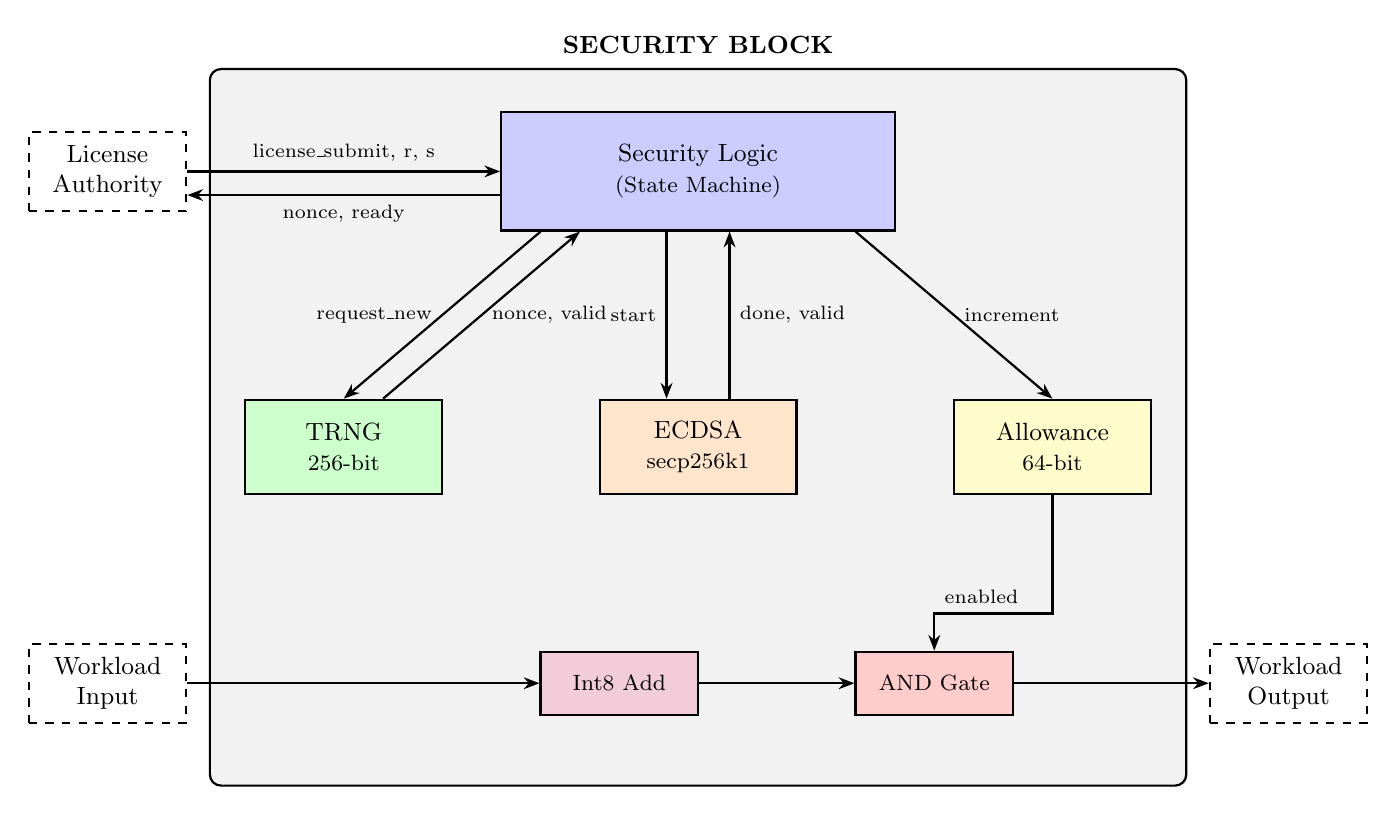
\begin{tikzpicture}[
    block/.style={rectangle, draw, thick, minimum width=2.5cm, minimum height=1.2cm, align=center, font=\small},
    smallblock/.style={rectangle, draw, thick, minimum width=2cm, minimum height=0.8cm, align=center, font=\footnotesize},
    external/.style={rectangle, draw, thick, dashed, minimum width=2cm, minimum height=1cm, align=center, font=\small},
    arrow/.style={-{Stealth[length=2mm]}, thick},
    label/.style={font=\scriptsize},
]

\node[block, fill=blue!20, minimum width=5cm, minimum height=1.5cm] (security) at (0, 0) 
    {Security Logic\\{\footnotesize (State Machine)}};

\node[block, fill=green!20] (trng) at (-4.5, -3.5) {TRNG\\{\footnotesize 256-bit}};
\node[block, fill=orange!20] (ecdsa) at (0, -3.5) {ECDSA\\{\footnotesize secp256k1}};
\node[block, fill=yellow!20] (allowance) at (4.5, -3.5) {Allowance\\{\footnotesize 64-bit}};

\node[smallblock, fill=purple!20] (adder) at (-1, -6.5) {Int8 Add};
\node[smallblock, fill=red!20] (andgate) at (3, -6.5) {AND Gate};

\node[external] (authority) at (-7.5, 0) {License\\Authority};
\node[external] (workload_in) at (-7.5, -6.5) {Workload\\Input};
\node[external] (workload_out) at (7.5, -6.5) {Workload\\Output};

\begin{scope}[on background layer]
    \draw[thick, rounded corners, fill=gray!10] 
        (-6.2, 1.3) rectangle (6.2, -7.8);
    \node[font=\small\bfseries] at (0, 1.6) {SECURITY BLOCK};
\end{scope}

\draw[arrow] ([xshift=-2cm]security.south) -- 
    node[label, left]{request\_new} (trng.north);
\draw[arrow] ([xshift=-0.4cm]security.south) -- 
    node[label, left]{start} ([xshift=-0.4cm]ecdsa.north);
\draw[arrow] ([xshift=2cm]security.south) -- 
    node[label, right]{increment} (allowance.north);
\draw[arrow] ([xshift=0.5cm]trng.north) -- 
    node[label, right]{nonce, valid} ([xshift=-1.5cm]security.south);
\draw[arrow] ([xshift=0.4cm]ecdsa.north) -- 
    node[label, right]{done, valid} ([xshift=0.4cm]security.south);
\draw[arrow] (allowance.south) -- ++(0, -1.5) -|
    node[label, above, pos=0.3]{enabled} (andgate.north);
\draw[arrow] (workload_in.east) -- (adder.west);
\draw[arrow] (adder.east) -- (andgate.west);
\draw[arrow] (andgate.east) -- (workload_out.west);
\draw[arrow] (authority.east) -- 
    node[label, above]{license\_submit, r, s} (security.west);
\draw[arrow] ([yshift=-0.3cm]security.west) -- 
    node[label, below]{nonce, ready} ([yshift=-0.3cm]authority.east);

\end{tikzpicture}
\caption{Security block architecture.}
\label{fig:architecture}
\end{center}
\end{figure}

Components:
\begin{itemize}[nosep]
    \item \textbf{TRNG}: 256-bit nonce generation (counter in prototype; ring oscillator in production)
    \item \textbf{ECDSA}: Signature verification on secp256k1
    \item \textbf{Allowance}: 64-bit counter, decrements every cycle, incremented by valid licenses
    \item \textbf{Output gating}: Each output bit ANDed with \texttt{enabled} signal
\end{itemize}

Outputs pass through only when authorized. Each bit is ANDed with \texttt{enabled}, which is high only when \texttt{allowance} $> 0$. The rest of the design ensures \texttt{allowance} increments only on presentation of a valid signature over the current nonce.

The state machine orchestrates the authorization flow:
\begin{enumerate}[nosep]
    \item TRNG generates a nonce
    \item Security block publishes nonce, asserts \texttt{nonce\_ready}
    \item External authority signs nonce, submits $(r, s)$
    \item ECDSA verifies signature against hardcoded public key
    \item If valid: allowance incremented, new nonce generated
    \item If invalid: allowance unchanged, same nonce retained (retry permitted)
\end{enumerate}

\iffalse
\begin{figure}[h]
\begin{center}
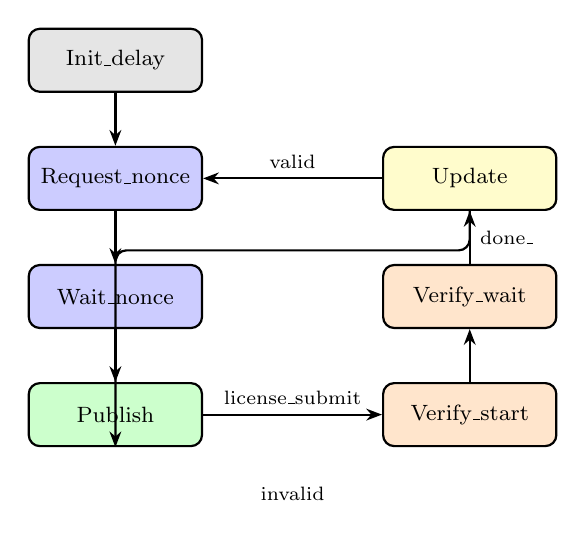
\begin{tikzpicture}[
    state/.style={rectangle, draw, thick, rounded corners, minimum width=2.2cm, minimum height=0.8cm, align=center, font=\footnotesize},
    arrow/.style={-{Stealth[length=2mm]}, thick},
    label/.style={font=\scriptsize},
]

\node[state, fill=gray!20] (init) at (0, 0) {Init\_delay};
\node[state, fill=blue!20] (request) at (0, -1.5) {Request\_nonce};
\node[state, fill=blue!20] (wait) at (0, -3) {Wait\_nonce};
\node[state, fill=green!20] (publish) at (0, -4.5) {Publish};
\node[state, fill=orange!20] (vstart) at (4.5, -4.5) {Verify\_start};
\node[state, fill=orange!20] (vwait) at (4.5, -3) {Verify\_wait};
\node[state, fill=yellow!20] (update) at (4.5, -1.5) {Update};

\draw[arrow] (init) -- (request);
\draw[arrow] (request) -- (wait);
\draw[arrow] (wait) -- (publish);
\draw[arrow] (publish) -- node[label, above]{license\_submit} (vstart);
\draw[arrow] (vstart) -- (vwait);
\draw[arrow] (vwait) -- node[label, right]{done\_} (update);
\draw[arrow] (update) -- node[label, above]{valid} (request);
\draw[arrow, rounded corners] (update.south) -- ++(0, -0.5) -- ++(-4.5, 0) -- ++(0, -0.5) -- (publish.south);
\node[font=\scriptsize] at (2.25, -5.5) {invalid};

\end{tikzpicture}
\caption{State machine transitions.}
\label{fig:statemachine}
\end{center}
\end{figure}

\fi

The ECDSA module (Figure \ref{fig:ecdsa}) verifies signatures by computing $R = u_1 \cdot G + u_2 \cdot Q$ and checking whether $R_x \equiv r \pmod{n}$.

\begin{figure}[h]
\begin{center}
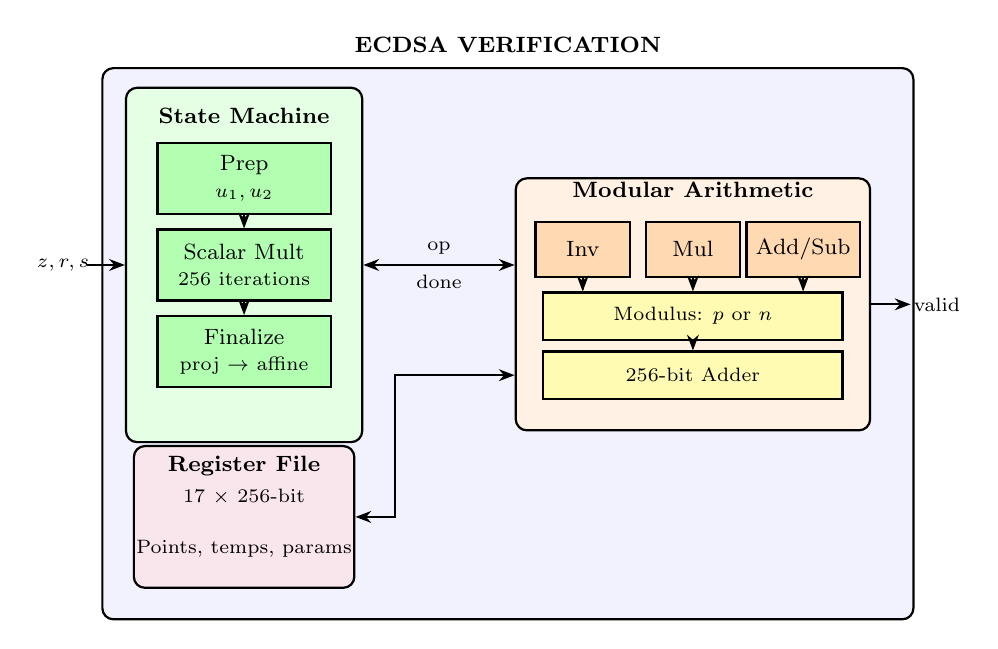
\begin{tikzpicture}[
    block/.style={rectangle, draw, thick, minimum width=2cm, minimum height=0.9cm, align=center, font=\footnotesize},
    container/.style={rectangle, draw, thick, rounded corners, fill=#1, minimum height=2cm},
    arrow/.style={-{Stealth[length=2mm]}, thick},
    biarrow/.style={{Stealth[length=2mm]}-{Stealth[length=2mm]}, thick},
    label/.style={font=\scriptsize},
]

% State Machine
\node[container=green!10, minimum width=3cm, minimum height=4.5cm] (sm_box) at (-3.2, 0) {};
\node[font=\footnotesize\bfseries] at (-3.2, 1.9) {State Machine};

\node[block, fill=green!30, minimum width=2.2cm] (prep) at (-3.2, 1.1) {Prep\\{\scriptsize $u_1, u_2$}};
\node[block, fill=green!30, minimum width=2.2cm] (loop) at (-3.2, 0) {Scalar Mult\\{\scriptsize 256 iterations}};
\node[block, fill=green!30, minimum width=2.2cm] (fin) at (-3.2, -1.1) {Finalize\\{\scriptsize proj $\to$ affine}};

\draw[arrow] (prep) -- (loop);
\draw[arrow] (loop) -- (fin);

% Register File
\node[container=purple!10, minimum width=2.8cm, minimum height=1.8cm] (reg_box) at (-3.2, -3.2) {};
\node[font=\footnotesize\bfseries] at (-3.2, -2.55) {Register File};
\node[font=\scriptsize] at (-3.2, -2.95) {17 $\times$ 256-bit};
\node[font=\scriptsize] at (-3.2, -3.6) {Points, temps, params};

% Arithmetic Unit
\node[container=orange!10, minimum width=4.5cm, minimum height=3.2cm] (arith_box) at (2.5, -0.5) {};
\node[font=\footnotesize\bfseries] at (2.5, 0.95) {Modular Arithmetic};

\node[block, fill=orange!30, minimum width=1.2cm, minimum height=0.7cm] (inv) at (1.1, 0.2) {Inv};
\node[block, fill=orange!30, minimum width=1.2cm, minimum height=0.7cm] (mul) at (2.5, 0.2) {Mul};
\node[block, fill=orange!30, minimum width=1.2cm, minimum height=0.7cm] (addsub) at (3.9, 0.2) {Add/Sub};

\node[block, fill=yellow!30, minimum width=3.8cm, minimum height=0.6cm] (mod) at (2.5, -0.65) {\scriptsize Modulus: $p$ or $n$};
\node[block, fill=yellow!30, minimum width=3.8cm, minimum height=0.6cm] (add256) at (2.5, -1.4) {\scriptsize 256-bit Adder};

\draw[arrow] (inv.south) -- ++(0, -0.15) -- (mod.north -| inv);
\draw[arrow] (mul.south) -- (mod.north);
\draw[arrow] (addsub.south) -- ++(0, -0.15) -- (mod.north -| addsub);
\draw[arrow] (mod) -- (add256);

% Connections
\draw[biarrow] (sm_box.east) -- node[label, above]{\scriptsize op} node[label, below]{\scriptsize done} (arith_box.west |- sm_box.east);
\draw[biarrow] (reg_box.east) -- ++(0.5, 0) |- (arith_box.west |- add256);

% External I/O
\node[font=\scriptsize] at (-5.5, 0) {$z, r, s$};
\draw[arrow] (-5.2, 0) -- (sm_box.west);
\draw[arrow] (arith_box.east) -- ++(0.5, 0);
\node[font=\scriptsize] at (5.6, -0.5) {valid};

% Outer box
\begin{scope}[on background layer]
    \draw[thick, rounded corners, fill=blue!5] 
        (-5, 2.5) rectangle (5.3, -4.5);
    \node[font=\footnotesize\bfseries] at (0.15, 2.8) {ECDSA VERIFICATION};
\end{scope}

\end{tikzpicture}
\caption{ECDSA verification module. The state machine orchestrates scalar multiplication using Shamir's trick (processing both $u_1$ and $u_2$ in a single pass). Point operations use complete addition formulas in projective coordinates.}
\label{fig:ecdsa}
\end{center}
\end{figure}

\subsection{Design Rationale}

\textbf{Deadman's switch}: The original paper \cite{petrie2025} argues that sending ``off'' signals to chips in unknown locations is unreliable. Chips may be air-gapped or shielded. Defaulting to off and requiring periodic re-authorization is more robust.

\textbf{Redundancy through distribution}: The full architecture calls for thousands of security blocks per chip. An attacker must bypass all of them. This prototype implements one block; duplication is straightforward.

\textbf{Public key cryptography}: Only the public key is stored on-chip. There is no secret to extract. The prototype hardcodes $Q = 2G$ for testing; production implementations would store chip-specific keys in Mask ROM.

\textbf{ECDSA verification}: The module uses Shamir's trick to compute $R = u_1 \cdot G + u_2 \cdot Q$ in a single pass through 256 bit positions. Each bit position requires one point doubling and one conditional addition, executed as a fixed 40-operation sequence. Point operations use complete addition formulas \cite{renes2016} in projective coordinates, where the point at infinity is $Z = 0$. This eliminates data-dependent branches, simplifying verification.

\textbf{Nonce rotation}: Invalid signatures return to Publish with the same nonce, allowing retry. Valid signatures trigger immediate nonce regeneration.

\textbf{Time-based depletion}: Allowance decrements every cycle rather than per-operation, ensuring expiration even during idle periods.

\section{Results}

\subsection{Artifacts}

Code and extended architecture documentation are available at \url{https://github.com/JamesPetrie/off-switch}.

\subsection{Simulation Results}

Simulation validates the following security properties:

\begin{itemize}[nosep]
    \item \textbf{Output gating}: When allowance reaches zero, outputs are forced to zero. When positive, computation proceeds normally.
    \item \textbf{Replay prevention}: After accepting a valid license, the block generates a new nonce. The same signature cannot be reused.
    \item \textbf{Fail-secure initialization}: Allowance starts at zero. Without a valid license, nothing works.
    \item \textbf{Invalid license handling}: Bad signatures do not affect allowance and do not change the nonce.
    \item \textbf{Cryptographic authorization}: Only signatures valid for the current nonce increment the allowance.
\end{itemize}

\section{Limitations}

\textbf{Prototype status}: This is a demonstration, not production-hardened code. Deployment would require thorough verification.

\textbf{Circuit size}: The original paper \cite{petrie2025} targeted roughly 10,000 gates per block. This prototype is substantially larger due to redundant arithmetic circuits, excess registers, and the additional state required by complete addition formulas. Optimization would be needed to approach the original target.

\textbf{Counter-based TRNG}: The prototype uses an incrementing counter for nonce generation. This is acceptable for testing, not deployment. The interface supports substituting a ring oscillator.

\textbf{Missing orchestration}: A real chip needs logic to collect nonces from thousands of blocks and distribute licenses. This prototype implements one block with direct external interfaces.

\textbf{Quantum vulnerability}: ECDSA will not survive capable quantum computers. Production systems should include alternative block designs using post-quantum cryptography, as \cite{petrie2025} suggests.

\section{Future Work}

\textbf{Verification}: The current test suite covers basic security properties. More thorough verification would include edge case testing, code review, and testing against malformed inputs.

\textbf{Formal verification}: The state machine has seven states and the security properties are enumerable. The use of complete addition formulas eliminates edge-case branches, and projective coordinates handle the point at infinity without special cases.

\textbf{Circuit optimization}: Sharing arithmetic circuits, reducing register count, and evaluating the size/verification tradeoff for complete formulas.

\textbf{Alternative designs}: The original paper proposes multiple independent block designs with different cryptographic assumptions, including post-quantum variants. Implementing alternatives would add defense in depth.

\textbf{Orchestration}: Building the on-chip infrastructure to manage thousands of blocks, possibly using existing microcontroller cores on AI accelerators.

\section{Conclusion}

This project built a working prototype of an embedded off-switch security block and documented its architecture. The implementation demonstrates the core authorization flow and security properties in simulation. While not yet production-ready, it provides a starting point for further development and security analysis.

\section*{Code}

\textbf{Repository}: \url{https://github.com/JamesPetrie/off-switch}

The ECDSA module predates the hackathon. The security block integration, state machine, TRNG interface, and documentation were developed during the hackathon.

\section*{LLM Usage}

Claude assisted with implementation, debugging, and drafting. Functionality was verified through simulation.

\begin{thebibliography}{9}

\bibitem{aarne2024}
Aarne, O., Fist, T., \& Withers, C. (2024).
Secure, governable chips: Using on-chip mechanisms to manage national security risks from AI \& advanced computing.

\bibitem{kulp2024}
Kulp, G., et al. (2024).
Hardware-enabled governance mechanisms: Developing technical solutions to exempt items otherwise classified under export control classification numbers 3a090 and 4a090.

\bibitem{petrie2024}
Petrie, J. (2024).
Near-term enforcement of AI chip export controls using a firmware-based design for offline licensing.

\bibitem{petrie2025}
Petrie, J. (2025).
Embedded Off-Switches for AI Compute.
\textit{arXiv preprint} arXiv:2509.07637.

\bibitem{renes2016}
Renes, J., Costello, C., \& Batina, L. (2016).
Complete addition formulas for prime order elliptic curves.
\textit{IACR Cryptology ePrint Archive}, 2015/1060.

\end{thebibliography}

\appendix

\section{Limitations \& Dual-Use Considerations}

\subsection{Technical Limitations}

\textbf{False security from insecure implementations}: A flawed implementation could give false confidence that chips are controlled when they are not. If the ECDSA verification has subtle bugs, or if the TRNG produces predictable nonces, attackers might forge valid licenses. This risk motivates the emphasis on formal verification and the use of complete addition formulas that eliminate edge cases.

\textbf{Accidental denial of service}: Bugs or operational failures could disable chips that should remain operational. If the licensing authority's systems fail, or if network connectivity is lost, legitimate users lose access to their hardware. The time-based allowance provides a buffer, but extended outages could still cause disruption. Production systems would need redundant licensing infrastructure and appropriate allowance periods.

\subsection{Dual-Use Risks}

\textbf{Concentration of power}: Hardware off-switches grant significant power to whoever controls the licensing keys. If a single entity controls authorization for a large fraction of global AI compute, that concentration could be misused for censorship, rent-seeking, or geopolitical coercion. Governance structures around key management would need careful design, potentially involving multiple independent parties or threshold signatures.

\textbf{Encouraging parallel supply chains}: If off-switches are mandated in some jurisdictions but not others, actors seeking ungovernable compute may invest in alternative chip fabrication. This could accelerate development of competing supply chains outside the reach of governance mechanisms, potentially worsening the problem the technology aims to solve.

\textbf{Sabotage and weaponization}: The same mechanism that allows legitimate authorities to disable chips could be exploited by attackers who compromise the licensing infrastructure. A compromised private key could disable chips globally. Conversely, state actors might use off-switches as a tool of economic warfare rather than safety governance.

\end{document}